\documentclass[12pt]{article}
\usepackage[utf8]{inputenc}
\usepackage{graphicx}
\usepackage{biblatex}
\usepackage{titlesec}
\usepackage{geometry}
\usepackage{setspace}
\usepackage{minted}
\usepackage{biblatex}
\usepackage{listings}

\geometry{
 a4paper,
 left=35mm,
 top=25mm,
 right=25mm,
 bottom=25mm,
 }
\setstretch{1.5}
\addbibresource{reference.bib}
\bibliography{reference}
\begin{document}
\graphicspath{{./pictures/}}
\titlelabel{\thetitle.\quad}
\renewcommand*\contentsname{Obsah}
\renewcommand{\bibfont}{\small}
\renewcommand{\thesection}{\Roman{section}} 
\renewcommand{\thesubsection}{\thesection.\Roman{subsection}}
\renewcommand{\thesubsubsection}{\thesubsection.\Roman{subsubsection}}
\renewcommand\listoflistingscaption{Seznam příloh}
\renewcommand{\listingscaption}{Příloha}
\begin{titlepage}
\begin{center}
    \vspace{2,5cm}
    \textbf{\Large Gymnázium, Praha 6, Arabská 14}\par
    \Large Obor Programování\par
    \vspace{2cm}
    \textbf{\Huge Ročníková práce}\par
    \vspace{2cm}
    \textbf{\Huge Custom Chess}\par
    \vspace{2cm}
    
\includegraphics[]{logo}\par
    \vfill
   \Large Petr Dobiáš, Josef Liška, Jakub Turek \hfill Duben 2023
   
    
     
\end{center}
\end{titlepage}
\newpage{}
\thispagestyle{empty}
\mbox{}
\vfill
Prohlašuji, že jsem jediným autorem tohoto projektu, všechny citace jsou řádně označené a všechna použitá literatura a další zdroje jsou v práci uvedené. Tímto dle zákona 121/2000 Sb. (tzv. Autorský zákon) ve znění pozdějších předpisů uděluji bezúplatně škole Gymnázium, Praha 6, Arabská 14
oprávnění k výkonu práva na rozmnožování díla (§ 13) a práva na sdělování díla veřejnosti (§ 18) na dobu časově neomezenou a bez omezení územního rozsahu.
\newline
V Praze dne \hfill Petr Dobiáš, Josef Liška, Jakub Turek
\newpage{}
\thispagestyle{empty}
\section*{Anotace}
Následující práce pojednává o vývoji aplikace založené na atchitektůře klient-server s využitím programovacích jazyku Java, Python a JavaScript, frameworku Django a databáze MongoDB, která umožnuje uživatelům vytvařet a následně hrát derivace hry šachy, v podobě úpravy figur, hrací desky a podmínek vítězství, online. Tyto derivace mohou uživatelé definovat ručně pomocí textovích soubru, či grafického návrháře v aplikaci. Aplikace se sestává ze serverové části a klientské webové aplikace.
\newpage
\setcounter{page}{1}
\tableofcontents 
\newpage
\section*{Úvod}
Následující práce pojednává o vývoji aplikace, jejímž cílem je umožnit uživatelům hrát v online multiplayeru derivace hry šachy a zároveň jim umožnit jednoduše tyto derivace vytvářet prostřednictvím grafického návrháře vlastních pravidel v klientské aplikaci. Přesná podoba těchto vlastních pravidel bude podrobněji rozebrána v následujících kapitolách, ale ve zkratce se jedná o možnost definovat vlastní rozměr šachovnice, rozložení figur nebo vytvoření vlastních figur a podobně.

Aplikace je založené na architektuře klient-server a skládá se tedy ze dvou částí. Serverové částí, která je napsaná v programovacím jazyku Java s využitím řady knihoven, kterým se budeme více věnovat později. A klientské části, kterou je v tomto případě webová aplikace, jejíž back-endová část je napsaná v jazyce Python s využitím frameworku Django, její front-endová část využívá CSS frameworku Bootstrap pro snazší práci s kaskádovými styly a JavaScriptové knihovny JQuery. Z tohoto důvodu bude tedy následující text rozdělen na dvě hlavní částy a to tedy na část pojednávající o serverové části aplikace a část pojednávající o klientské části aplikace.
\addcontentsline{toc}{section}{Úvod}
\newpage
\section{Tvorba vlastních pravidel hry šachy}
\newpage
\section{Server}
Následující kapitola pojednává o serverové části aplikace, tedy o její struktuře, technologiích použitých pro její vývoj, řešení některých klíčových problémů řešených v této části aplikace a také o komunikačním protokolu sloužícímu pro komunikaci mezi serverem a klientem.
\subsection{Použité technologie}
Následující kapitola poskytuje výčet technologií a knihoven používaných serverem a stručný popis jejich fungování a využití v tomto projektu
\subsubsection{MongoDB}
Jedná se on o NoSQL, což znamená, že místo klasické struktury tabulek známe z SQL databází, jsou data ukládána do souboru BSON, binární forma formátu JSON, což usnadňuje například ukládání souboru. Databázi je také možno v rámci služby Atlas provozovat v cloudu bez nutnosti vetší údržby, což je možnost, kterou využívá i tento projekt. Pro komunikaci s touto databází serverová část používat také MongoDB driver pro jazyk Java a také knihovnu Morphia, která poskytuje obdobu objektově orientovaného mapování pro NoSQL databázi MongoDB.
\subsubsection{Bouncy castel}
Jedná se o opensource knihovnu, která nabízí implementace většiny standartě používaných kryptografických algoritmů v jazyce Java\cite{bouncyCastle}. V tomto projektu je primárně využívána pro zabezpečení komunikace mezi klientem a serverem pomocí protokolu TLS 1.3, ale také pro bezpečné ukládání hesel do databáze ve standartu podporované Django frameworkem.
\subsubsection{Simple Java Mail a Jsoup}
Jedná se o knihovnu, která usnadňuje odesílání emailů pomocí Javy, kdy po prvotním nakonfigurování STMP serveru, případně dalších parametrů jako například šifrování zpráv, umožňuje jednoduše odesílat jak prosté textové zprávy, tak emaily definované pomocí HTML šablony. Právě druhá z možností je využívána v tomto projektu a pro dynamické vkládání dat, jako třeba url pro reset hesla, do HTML šablon je používána druhá ze zmíněných knihoven, HTML parser Jsoup. Obě tyto knihovny jsou tedy v tomto projektu využívány  pro odesílání emailu pro potvrzení registrace a případně reset hesla.
\subsubsection{Gson}
Knihovna vytvořená společností Google sloužící pro serializaci Java objektů do podoby textového řetězce ve formátu json. Slouží jednak pro načítání vlastních pravidel hry, která jsou uložena v několika souborech ve formátu json a také pro serializaci dat, které jsou během hry odesílaný serverem klientu pro zobrazení, jako aktuální rozložení figur a podobně.
\newpage
\subsection{Struktura aplikace a základy fungování}
Následující podkapitola se věnuje struktuře serverové aplikace a základním principům jejího fungování. Server je rozdělen na dva balíčky první z nich Connection, jak už název napovídá, se stará o síťovou komunikaci a autentizaci klientu, zatím co druhý balíček GameLogic, obstarává samotný průběh hry, tedy interpretaci vlastních pravidel hry a vyhodnocovaní tahů zahraných hráči. Následující dvě sekce, tedy stručně pojednávají o struktuře a fungování každého z těchto balíčků. 
\subsubsection{Connection}
Z hlediska funkce by se třídy tohoto balíčku dali rozdělit do pěti základních kategorií. Tyto kategorie a některé do nich spadající třídy budou zmíněny v následujícím stručném schnutí fungování aplikace, ale kompletní seznam tříd a jejich zařazení můžete najít v přiložené tabulce.

Po spuštění serveru dojde k načtení jeho konfigurace ze souboru \textit{config.json}, kde je specifikovaná, délka fronty, maximální počet připojených klientů, ale třeba také cesta k SSL certifikátu a privátnímu klíčí, který slouží pro zabezpečení komunikace, či STMP serveru pro odesílaní verifikačních emailu.

Poté je spuštěno hlavní vlákno serveru reprezentované třídou \textit{Server}, které je zodpovědné za navazování spojení s klientem a následné zařazení tohoto spojení buďto mezi obsluhované klienty, nebo, v případě překročení kapacity serveru, do fronty a také pomocné vlákno, reprezentované třídou \textit{}{QueueManager}, které je zodpovědné za správu fronty, tedy za odstraňování zavřených spojení z fronty, či zařazování spojení z fronty mezi obsluhovaná po uvolnění kapacity. Obě tyto třídy patří mezi vlákna režie, která jsou jak je již patrno za správu jednotlivcích spojení, či prostředků aplikace.

Pokud je na serveru ještě volná kapacita, dojde po zařazení spojení mezi obsluhovaná připojení je pro jeho obsluhu vytvořeno nové vlákno reprezentované třídou \textit{ClientThread} a je zahájena autentizační rutina, která neskončí dokud se uživatel úspěšně nepřihlásí nebo se nedojde k ukončení spojení. Pokud je autentizace úspěšně dokončena začne vlákno obsluhovat požadavky klienta, do doby dokud klient nevytvoří novou hru, nebo se nepřipojí do již existující hry. Protokol této komunikace bude popsán v další kapitole.

Ve chvíli kdy se uživatel připojí do hry, dojde k odeslání souboru potřebných pro danou hru, vlastní ikony figur, z databáze klientovi. Poté dojde k ukončení daného vlákna a komunikace začne být obsluhována vláknem reprezentovaným třídou \textit{GameThread}, které spravuje komunikaci mezi všemi hráči v jedné hře, hra probíhá na tahy, tudíž je žádoucí aby byli klienti obsluhování postupně. Vlákno \textit{GameThread} začne vyhodnocovat požadavky až po připojení všech hráčů. Třídy \textit{GameThread} a \textit{ClientThread} tedy patří mezi komunikační vlákna, jejich hlavním účelem je přijímat požadavky od klientu, spouštět příslušné metody pro jejich obsluhu a odesílání výsledků v podobě odpovědi.

Po záhejení hry už je pouze s pomocí tříd balíčku GameLogic v smyčce vyhodnocovány tahy jednotlivých hráčů a jsou jim vraceny jejich výsledky do doby, než je hra ukončena. V tuto chvíli je hráčum odeslán výsledek hry a \textit{GamesManager} odebere dohranou hru ze seznamu probíhajících her a komunikace s jednotlivými hráči je opět přesunuta do samostatných vláken.

Zbylé tři skupiny, o kterých jsem se v rámci popisu fungování balíčku nezmínil jsou třídy sloužící pro reprezentaci dat v databázi, které jsou používány pro objektově relační mapování dat v databázi. Třídy datových objektů, které jsou podobné předchozí skupině s tím rozdílem, že obsahují i data, které jsou potřeba pouze za běhu programu a není třeba je ukládat. Poslední skupinou jsou třídy s logikou, které obsahují pouze třídu \textit{Game}, která definuje průběh herní smyčky ve vlákně \textit{GameThread}.
\begin{listing}[!ht]
\begin{tabular}{ |p{3cm}|p{3,2cm}|p{3,2cm}|p{4cm}| }
\hline
\multicolumn{4}{|c|}{Rozaření tříd dle funkce} \\
\hline
 Vlákna režie& Pomocné třídy & Datové objekty & Databázová data \\
\hline
Server & Sender &Client &ClientDataObject\\
GamesManager & Reciever  & ServerParameters &  GameDataObject\\
\cline{3-3} QueueManager&EmailSender& Třídy s logikou & AuthenticationToken   \\
\cline{1-1} \cline{3-3} Komunikační vlákna & ParametersParser PasswordHasher & Game & FigureDataObject \\
\cline{1-1} ClientThread GameThread& SecureConnection Manager& &\\
& UserAuthenticator & &\\
\hline
\end{tabular}
\caption{Tabulka reprezentující rozřazení tříd balíčku Connection dle funkce}
\end{listing}
\
\newpage
\subsubsection{GameLogic}
\newpage
\subsection{Klíčové problémy a jejich řešení}
Následující kapitola pojednává o nejzásadnějších problémech, které bylo třeba na straně serveru vyřešit a popisuje jejich případné řešení.
\subsubsection{Komunikační protokol}
Jedním z klíčových problému aplikace bylo vytvořit efektivní a snadno použitelný systém komunikace mezi serverem a klientem. Pro tento účel jsem tedy vytvořili jednoduchý textový komunikační protokol, kdy se požadavek vždy skládá ze jména požadavku a jeho argumentů oddělených dvojtečkami. Následující ukázka kód tedy ukazuje vytvoření obecného požadavku a následně i konkrétní požadavek pro přihlášení. 
\begin{listing}[!ht]
\begin{minted}{python}
# obecný požadavek
request = 'rquest_name:arg1:arg2'
# příklad požadavku o autentikaci
# zjednodušeně znázorněné odeslání a přijetí dat
server_connection.send('signin:username:password') 
response = server_connection.reciece().split(':')
if(response[1] == 'success'):
    print('přihlášen')
else:
    print(response[1])  
\end{minted}
\caption{Ukázka vytvoření požadavku protokolu v jazyce Python}
\end{listing}
Jak je vidět z výše uvedeného příkladu, tak odpověď serveru na požadavek je v případě požadavku na provedení akce na serveru buďto \textit{msg:success} v případě úspěšného provedení,nebo \textit{err:error message} v případě selhání. Nebo v případě, že se jedná o požadavek o zaslání dat, zůstává chybová odpověd stejná, ale v případě úspěchu jsou navrácena požadovaná data ve formátu json.

Pro vysvětlení fungování protokolu následující tabulka uvádí všechny možné požadavky, seznam jejich argumentů (je třeba je zadat v uvedeném pořadí) a typ jejich odpovědi.
\newpage
\begin{listing}[!ht]
\begin{tabular}{ |p{4cm}|p{6cm}|p{4cm}| }
\hline
název požadavku & argumenty & návratová hodnota \\
\hline
signin & username, password & None \\
signup & username, password, email & None\\
reset & username/email & None\\
crtg & game name, password, rules name & None\\
joig & game name, password & array of images \\
getg & None & array of games names\\
getr & None & array of rules names\\
\hline
\end{tabular}
\caption{Seznam všech požadavků a jejich argumentů}
\end{listing}
\subsubsection{Znovu připojení do hry}
Další zásadní problémem byla nutnost vyřešit způsob, jak umožnit hráči, který v době kdy se účastní hry ztratí spojení se serverem, znovu se připojit do rozehrané hry a dohrát ji.

Řešení tohoto problému se nakonec ukázalo jako ne tak komplikované, jak by se na první pohled mohlo zdát. Pro implementaci této mechaniky totiž stačí používat unikátní identifikátory pro každé připojení do hry, které jsou v našem případě reprezentovány náhodným textovým řetězcem.

Vzhledem k tomu, že běžící server si uchovává informace o připojených klientech ve formě instancí třídy \textit{Client}, je možné vždy při připojení do nové hry do této instance uložit, náhodně vygenerovaný textový řetězec, jeho generování je znázorněno v ukázce níže, a zároveň tento identifikátor uložit pro daného uživatele do databáze.

\begin{listing}[!ht]
\begin{minted}{java}
 private String getRandomString(int size) {
        byte[] stringBytes = new byte[size];
        new Random().nextBytes(stringBytes);
        return new String(Base64.encodeBase64(stringBytes));
}
\end{minted}
\caption{Generování náhodného řetězce v jazyce Java}
\end{listing}

Po implementování těchto identifikátorů už jen stačí pokaždé, když je navázáno nové spojení s klientem získat z databáze tento identifikátor, a pokud se shoduje s identifikátorem některého z odpojených hráčů, jednoduše spoji toto nové připojení s daty o daném hráči.

Poté už stačí jen kdykoliv, kdy dojde ke ztrátě spojení, místo ukončení hry pouze označit daného hráče za odpojeného a spustit timeout po jehož vypršení dojde ke kontrole zda se daný hráč znovu připojil a pokud ano, je mu odeslán aktuální stav hry a hra pokračuje, v opačném případě je hra ukončena.
\subsubsection{Autentizace klientů}
Dalším ze zásadních problémů bylo při spuštění ověřit identitu uživatele a zobrazit mu pouze jemu náležící data, a tedy v podstatě vytvořit uživatelské účty.

Vyřešit tento problém nebylo zdaleka tak náročné, jelikož se jedná o jeden z nejčastěji řešených problémů a je jeho řešení je tedy velmi dobře zdokumentované a má jasně formulované postupy dobré praxe, kterých se držet pro vytvoření bezpečných uživatelských účtů. Tento projekt využívá pro ukládání hesel standard užívaného frameworkem Django a to z důvodu snazšího procesu změny hesla, která je dokončována právě webovou aplikací napsanou s pomocí Django frameworku. Nyní tedy přejděme k samotnému procesu vytvoření uživatelského účtu.

Poté, co uživatel zašle požadavek o vytvoření nového účtu, dojde k ověření zda-li pro zadaný email a jméno již účet neexistuje a pokud ne, jsou zadané údaje uloženy do databáze jakožto nový uživatelský účet, který ale zatím není aktivovaný a nemůže se pomocí něj nikdo přihlásit. Proto aby byl účet aktivován, je nejprve nutné ověřit zadaný email, pomocí odkazu, který byl na tento email zaslán. Tento odkaz vede na webovou aplikaci, která se stará o ověřování uživatelských účtu a jako base64 je v něm zakódované id daného uživatele a hodnota autentizačního tokenu, který je vygenerován při vytvoření účtu a tvoří ho hodnota, kterou představuje náhodný řetěze, který je generován jako v předchozím případě akorát s využitím kryptograficky bezpečného náhodného čísla a data expirace, které je nastaveno na den po vygenerování. Hash jeho hodnoty a datum expirace je uloženo pro daný účet do databáze. Po otevření zaslané adresy z ní tedy webová aplikace získá id uživatele a hodnotu autentizačního tokenu, následně tedy spočítá hash získané hodnoty a zjistí zdali je pro uživatele s daným id v databázi uložený platný token hash jehož hodnoty by odpovídal vypočítanému hashy, pokud ano je účet aktivován, token odstraněn z databáze a uživatel se může přihlásit, v opačném případě se mu zobrazí chybová hláška a účet zůstane neaktivní.

Pokud se uživatel přihlašuje pomocí již existujícího účtu, je na server poslán požadavek, který obsahuje uživatelem zadané uživatelské jméno, nebo email a heslo. V tomto případě je v databázi jednoduše vyhledán uživatel s daným emailem, nebo jménem a jsou získány informace s jakým algoritmem, saltem a počtem iterací byl vypočítán hash jeho hesla uložený v databázi a s pomocí těchto údajů je vypočítán hash hesla zaslaného v požadavku, pak už stačí oba hashe porovnat a v případě, že se shodují je uživatel přihlášen.

Pokud uživatel zažádá o změnu hesla, je průběh téměř totožný aktivaci nového účtu, s tím rozdílem, že po úspěšném ověření webová aplikace uživatele vyzve k zadání nového hesla, vygeneruje pro něj nový salt a s jeho pomocí spočítá hash nového hesla, tyto informace jsou následně uloženy do databáze a uživatel se může přihlást pomocí nového hesla. 

\subsubsection{Ukládání dat do databáze}
Jedním z posledních problémů, které bylo třeba vyřešit, bylo jak reprezentovat uživatelská dat v databázi. Pro demonstraci toho, jaká data jsou v databázi uloženy a jaké jsou mezi nimi vztahy, slouží následující schema, pro jehož použití jsem se rozhodl, i přesto že MongoDB nemá na rozdíl od SQL databází nic jako fixní schéma, ale považoval jsem ho za vhodnější formu popisu uložených dat než slovní popis, zároveň bych chtěl ještě dodat, že pole souborů by samozřejmě opět šlo rozepsat jako one-to-many relation mezi výchozí kolekcí a kolekcí file, ale vzhledem k tomu, že kolekce file je vytvářena samotnou databází, rozhodl jsem se použít toto zjednodušení.
\begin{listing}[!ht]
 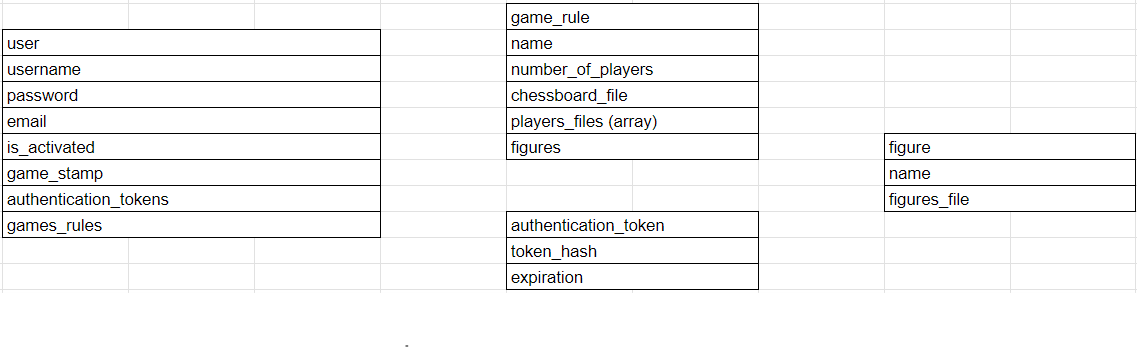
\includegraphics[scale=0.75, width=15cm]{pictures/schem.png}\par
\caption{Schéma databáze}
\end{listing}
\newpage
\section{Klient}
Lorem ipsum dolor sit amet, consectetur adipiscing elit. Donec auctor, nisl eget aliquam aliquam, nunc nisl aliquet nisl, eget aliquet
\newpage
\printbibliography[heading=bibintoc,title={Reference}]
\newpage
\addcontentsline{toc}{section}{Seznam příloh}
\listoflistings


\end{document}
